\documentclass{article}


\setcounter{tocdepth}{5}
\usepackage[subpreambles=true]{standalone}
\usepackage[utf8]{inputenc}
\usepackage[english]{babel}

\usepackage{import}
\usepackage{hyperref}
\usepackage[toc]{glossaries}
\usepackage{graphicx}
\usepackage{listings}
\usepackage{color}

\definecolor{dkgreen}{rgb}{0,0.6,0}
\definecolor{gray}{rgb}{0.5,0.5,0.5}
\definecolor{mauve}{rgb}{0.58,0,0.82}

\lstset{
    frame=tb,
    language=Java,
    aboveskip=3mm,
    belowskip=3mm,
    showstringspaces=false,
    columns=flexible,
    basicstyle={\small\ttfamily},
    numberstyle=\color{gray},
    keywordstyle=\color{blue},
    commentstyle=\color{dkgreen},
    stringstyle=\color{mauve},
    breaklines=true,
    breakatwhitespace=true,
    numbers=left,
    stepnumber=1,
    % numbersep=5pt,
    tabsize=2
}

% Define variables for the "\maketitle" command
\title{Leistungsnachweis im Fach Programmierung 1}
\date{2020-12-07 - 2020-01-17}
\author{Maximilian von Hohenbühel \\ Fabian Cieslik}
% Define the glossary
\makeglossaries
\begin{document}
\pagenumbering{Roman}
\maketitle
\newpage
\tableofcontents % Show structure of all sections and paragraphs
\newpage

\section{Projektvorraussetzungen}
\textbf{Beschreibung:} Die Projektaufgabe besteht darin, ein einfaches Spiel zu implementieren. Die Wahl des Spiels bleibt Ihnen überlassen, beachten Sie jedoch, dass sich im Rahmen von 36 Stunden Arbeitszeit nur sehr begrenzte Spielideen auch umsetzen lassen.
\newline
\textbf{Details:} Sie programmieren ein Spiel für ein sehr eingeschränktes Display. Dieses enthält nur $24\times 48$ Bildpunkte (Pixel), d.h. 24 Reihen mit jeweils 48 Spalten. Jeder Bildpunkt kann 16 Millionen Farben annehmen, wobei die Rot, Grün und Blau-Komponente mit jeweils einem Byte angesprochen wird. Als Steuermöglichkeit stehen Ihnen vier Tasten zur Verfügung, die wie im Cursorblock üblich angeordnet sind. Es gibt nur einen Spieler. Die Zeit für eine Spielrunde sollte bei 20-30 Sekunden liegen.
\newline
Zur Ein- und Ausgabe erhalten Sie eine Klasse mit zwei Methoden:
\begin{itemize}
    \item \textit{public int getKeyboard()}
        \newline
        Liefert die vier Cursortasten der Tastatur folgende Werte zurück:
        \newline - 0 -$>$ "hoch"
        \newline - 1 -$>$ "runter"
        \newline - 2 -$>$ "links"
        \newline - 3 -$>$ "rechts"
        \newline - -1 -$>$ keine Taste
    \item \textit{public void showImage(short[] image)}
        \newline
        Zeigt ein komplettes Bild auf dem Display an, wobei der erste Wert des Arrays die Rot-Komponente des linken oben Bildpunkts ist und der letzte Wert die Blau-Komponente von 0 bis 255 des rechten unteren Bildpunktes. Das übergebene Array muss exakt $24*48*3$ Elemente haben für die 24 Zeilen, 48 Spalten und 3 Farbkomponenten pro Pixel. Das Display wird zeilenweise durchlaufen.
\end{itemize}
\textbf{Spielumfang:}
\begin{itemize}
    \item Eine \textit{interaktive Spielerfigur}
    \item Eine \textit{automatisch gesteuerte Spielerfigur}
    \item Einen Hintergrund
    \item Ein \textit{Score-System}
    \item Ein \textit{Highscore-System}
    \item Implementierungsvorgaben:
        \newline - Eine generische Klasse
        \newline - Drei davon abgeleitete Klassen (Spieler, Hintergrund, Gegner/NPC)
\end{itemize}
\newpage

\section{Idee}
\textbf{Name:}
\newline
MP - Mari proelium
\newline
\textbf{Spiel:}
\newline
Der Spieler steuert ein Schiff und probiert so lang zu überleben wie möglich. Es existieren Gegner, die sich zufällig bewegen.
\newline
Das Spiel wird in einer Vogelperspektive gespielt, man hat dadurch jederzeit den Überblick der gesamten Karte.
\newline
Das Spielprinzip der Runden wird in dem Sinne implementiert, dass alle 30 Sekunden neue Gegner auftauchen und man für jede überlebte Runde zusätzliche Punkte bekommt.
\newline
Das Punktesystem wird von der Zeit, die man am Leben ist und der Anzahl der besiegten feindlichen Schiffe beeinflusst.
\newline
Die Steuerung wird auf die vier verfügbaren Tasten aufgeteilt, sodass man ohne Probleme sein Schiff steuern kann und zugleich auch schiessen kann. Die Kollisionsinteraktionen mit feindlichen Schiffen und eventuellen Häfen wird vom System übernommen.
\newpage

\section{Beschreibung}
\textbf{Karte:}
\begin{itemize}
    \item \textbf{Aussehen}
        \newline
        Die Karte hat einen blauen Hintergrund, der den Ozean darstellt. Auf dem Ozean kann es vorkommen, dass es verschiedene Inseln geben kann. Inseln werden durch braune Pixel dargestellt. Die Platzierung der Inseln wird zufällig am Anfang des Spiels festgelegt und wird nur bei einem kompletten Neustart verändert. Auf den Inseln können Häfen generiert werden, die einem einen Bonus geben, falls man sie erreichen sollte. Die Häfen können vom Spieler und den Gegnern eingenommen werden und helfen der dementsprechenden Partei.
\end{itemize}
\textbf{Spieler:}
\begin{itemize}
    \item \textbf{Aussehen}
        \newline
        Ein zwei bzw. drei Pixel langes Schiff.
    \item \textbf{Fähigkeiten}
        \newline - Links: 45 Grad Drehung gegen den Uhrzeigersinn
        \newline - Rechts: 45 Grad Drehung in den Uhrzeigersinn
        \newline - Oben: Vorwärts Bewegung nach vorne
        \newline - Unten: Benutzen der Schiffsinternen Kanone
\end{itemize}
\textbf{Gegner:}
\begin{itemize}
    \item \textbf{Aussehen}
        \newline
        Ein zwei bzw. drei Pixel langes Schiff.
    \item \textbf{Fähigkeiten}
        \newline - Zufälliges Bewegen auf der Karte
        \newline - Bei Spielersicht wird Geschossen
\end{itemize}
\textbf{Punkte:}
\begin{itemize}
    \item \textbf{Punktequellen}
        \newline - Beim treffen eines Gegners
        \newline - Beim besiegen eines Gegners
        \newline - Besiegen aller gerade lebender Geger
        \newline - Fürs überleben einer Runde
    \item \textbf{Highscore}
        \newline
        Punkte werden in der Konsole als Highscore nach jedem Tod des Spielers ausgegeben
\end{itemize}
\newpage

\section{Programmablauf}
\begin{itemize}
    \item \textbf{Vorbereitung}
        \newline
        Es werden alle Spielnotwendigen Variablen deklariert und initialisiert. In einer \textit{Do-While} Schleife wird daraufhin gestarted um mehrere Spiele hintereinander spielen zu Können. Am Start der Schleife wird die Karte, der Spieler und die Gegner erstellt und gezeichnet und auf eine Eingabe des Benutzers gewartet. Bei Eingabe wird der Spielablauf gestartet. Nach dem Tod des Spielers wird der Punktestand ausgegeben und die Möglichkeit geboten ein neues Spiel zu Starten.
    \item \textbf{Spielablauf}
        \newline
        Zuerst wird der Spieler bewegt und auf Kollisionen überprüft, danach die Gegner. Anschließend wird überprüft ob man eine Runde überlebt hat.
\end{itemize}
\newpage

\section{Klassendiagramm}
\newline
\textbf{Hier sehen Sie einen groben Ausschnitt des Klassendiagramms der die Vererbung der Klassen darstellt. Die ausführliche Version des Klassendiagramms können Sie im \textit{Documentation} Ordner finden.}
\newline

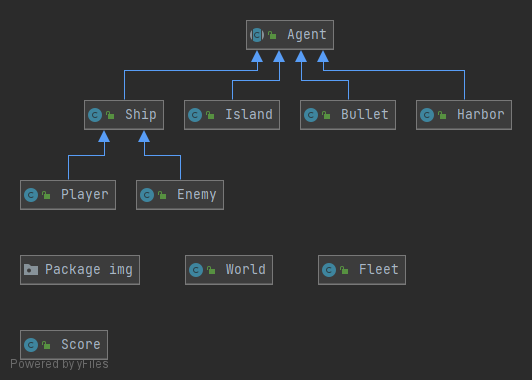
\includegraphics[width=\textwidth,height=\textheight,keepaspectratio]{./images/Rough_UML.png}
\newpage
\section{Programmcode}
\textbf{Ship.java}
\lstinputlisting{../Game/src/de/thdeg/game/assets/Ship.java}
\newpage
\textbf{Agent.java}
\lstinputlisting{../Game/src/de/thdeg/game/assets/Agent.java}
\newpage
\textbf{Enemy.java}
\lstinputlisting{../Game/src/de/thdeg/game/assets/Enemy.java}
\newpage
\textbf{Fleet.java}
\lstinputlisting{../Game/src/de/thdeg/game/assets/Fleet.java}
\newpage
\textbf{Bullet.java}
\lstinputlisting{../Game/src/de/thdeg/game/assets/Bullet.java}
\newpage
\textbf{Harbor.java}
\lstinputlisting{../Game/src/de/thdeg/game/assets/Harbor.java}
\newpage
\textbf{Island.java}
\lstinputlisting{../Game/src/de/thdeg/game/assets/Island.java}
\newpage
\textbf{Player.java}
\lstinputlisting{../Game/src/de/thdeg/game/assets/Player.java}
\newpage
\textbf{GameMain.java}
\lstinputlisting{../Game/src/de/thdeg/game/assets/GameMain.java}
\newpage
\textbf{World.java}
\lstinputlisting{../Game/src/de/thdeg/game/assets/World.java}
\newpage
\textbf{Score.java}
\lstinputlisting{../Game/src/de/thdeg/game/assets/Score.java}
\end{document}
